%
% ---------------------------------------------------------------
% Copyright (C) 2012-2018 Gang Li
% ---------------------------------------------------------------
%
% This work is the default powerdot-tuliplab style test file and may be
% distributed and/or modified under the conditions of the LaTeX Project Public
% License, either version 1.3 of this license or (at your option) any later
% version. The latest version of this license is in
% http://www.latex-project.org/lppl.txt and version 1.3 or later is part of all
% distributions of LaTeX version 2003/12/01 or later.
%
% This work has the LPPL maintenance status "maintained".
%
% This Current Maintainer of this work is Gang Li.
%
%

\documentclass[
 size=14pt,
 paper=smartboard,  %a4paper, smartboard, screen
 mode=present, 		%present, handout, print
 display=slides, 	% slidesnotes, notes, slides
 style=tuliplab,  	% TULIP Lab style
 pauseslide,
 fleqn,leqno]{powerdot}


\usepackage{cancel}
\usepackage{caption}
\usepackage{stackengine}
\usepackage{smartdiagram}
\usepackage{attrib}
\usepackage{amssymb}
\usepackage{amsmath} 
\usepackage{amsthm} 
\usepackage{mathtools}
\usepackage{rotating}
\usepackage{graphicx}
\usepackage{boxedminipage}
\usepackage{rotate}
\usepackage{calc}
\usepackage[absolute]{textpos}
\usepackage{psfrag,overpic}
\usepackage{fouriernc}
\usepackage{pstricks,pst-3d,pst-grad,pstricks-add,pst-text,pst-node,pst-tree}
\usepackage{moreverb,epsfig,subfigure}
\usepackage{color}
\usepackage{booktabs}
\usepackage{etex}
\usepackage{breqn}
\usepackage{multirow}
\usepackage{natbib}
\usepackage{bibentry}
\usepackage{gitinfo2}
\usepackage{siunitx}
\usepackage{nicefrac}
%\usepackage{geometry}
%\geometry{verbose,letterpaper}
\usepackage{media9}
\usepackage{animate}
%\usepackage{movie15}
\usepackage{auto-pst-pdf}

\usepackage{breakurl}
\usepackage{fontawesome}
\usepackage{xcolor}
\usepackage{multicol}



\usepackage{verbatim}
\usepackage[utf8]{inputenc}
\usepackage{dtk-logos}
\usepackage{tikz}
\usepackage{adigraph}
%\usepackage{tkz-graph}
\usepackage{hyperref}
%\usepackage{ulem}
\usepackage{pgfplots}
\usepackage{verbatim}
\usepackage{fontawesome}


\usepackage{todonotes}
% \usepackage{pst-rel-points}
\usepackage{animate}
\usepackage{fontawesome}

\usepackage{listings}
\lstset{frameround=fttt,
frame=trBL,
stringstyle=\ttfamily,
backgroundcolor=\color{yellow!20},
basicstyle=\footnotesize\ttfamily}
\lstnewenvironment{code}{
\lstset{frame=single,escapeinside=`',
backgroundcolor=\color{yellow!20},
basicstyle=\footnotesize\ttfamily}
}{}


\usepackage{hyperref}
\hypersetup{ % TODO: PDF meta Data
  pdftitle={Presentation Title},
  pdfauthor={Gang Li},
  pdfpagemode={FullScreen},
  pdfborder={0 0 0}
}


% \usepackage{auto-pst-pdf}
% package to show source code

\definecolor{LightGray}{rgb}{0.9,0.9,0.9}
\newlength{\pixel}\setlength\pixel{0.000714285714\slidewidth}
\setlength{\TPHorizModule}{\slidewidth}
\setlength{\TPVertModule}{\slideheight}
\newcommand\highlight[1]{\fbox{#1}}
\newcommand\icite[1]{{\footnotesize [#1]}}

\newcommand\twotonebox[2]{\fcolorbox{pdcolor2}{pdcolor2}
{#1\vphantom{#2}}\fcolorbox{pdcolor2}{white}{#2\vphantom{#1}}}
\newcommand\twotoneboxo[2]{\fcolorbox{pdcolor2}{pdcolor2}
{#1}\fcolorbox{pdcolor2}{white}{#2}}
\newcommand\vpspace[1]{\vphantom{\vspace{#1}}}
\newcommand\hpspace[1]{\hphantom{\hspace{#1}}}
\newcommand\COMMENT[1]{}

\newcommand\placepos[3]{\hbox to\z@{\kern#1
        \raisebox{-#2}[\z@][\z@]{#3}\hss}\ignorespaces}

\renewcommand{\baselinestretch}{1.2}


\newcommand{\draftnote}[3]{
	\todo[author=#2,color=#1!30,size=\footnotesize]{\textsf{#3}}	}
% TODO: add yourself here:
%
\newcommand{\gangli}[1]{\draftnote{blue}{GLi:}{#1}}
\newcommand{\shaoni}[1]{\draftnote{green}{sn:}{#1}}
\newcommand{\gliMarker}
	{\todo[author=GLi,size=\tiny,inline,color=blue!40]
	{Gang Li has worked up to here.}}
\newcommand{\snMarker}
	{\todo[author=Sn,size=\tiny,inline,color=green!40]
	{Shaoni has worked up to here.}}

%%%%%%%%%%%%%%%%%%%%%%%%%%%%%%%%%%%%%%%%%%%%%%%%%%%%%%%%%%%%%%%%%%%%%%%%
% title
% TODO: Customize to your Own Title, Name, Address
%
\title{Predict Future Sales}
\author{
Siyu Chen
\\
\\Xi'an Shiyou University

}
\date{\gitCommitterDate}


% Customize the setting of slides
\pdsetup{
% TODO: Customize the left footer, and right footer
rf=\href{http://www.tulip.org.au}{
Last Changed by: \textsc{\gitCommitterName}\ \gitVtagn-\gitAbbrevHash\ (\gitAuthorDate)
},
cf={Group Outlying Aspects Mining},
}


\begin{document}

\maketitle

%\begin{slide}{Overview}
%\tableofcontents[content=sections]
%\end{slide}


%%==========================================================================================
%%
\begin{slide}[toc=,bm=]{Overview}
\tableofcontents[content=currentsection,type=1]
\end{slide}
%%
%%==========================================================================================


\section{Problem Definition}


%%==========================================================================================
%%
\begin{slide}{Analyze Data}
\begin{center}
\twotonebox{\rotatebox{90}{Defn}}{\parbox{.86\textwidth}
{predict total sales for every product and store in the next month.
\begin{itemize}
\item sales_train.csv: Training set (2013 to October 2015)
\item test.csv: Test set (Forecast sales of these stores and products in November 2015)
\item sample_submission.csv: A properly formatted sample submission file
\item items.csv: Additional information about the merchandise/product
\item item_categories.csv: Additional information on the categories of goods
\item shops.csv: Additional information about the store
\end{itemize}
}}

\end{center}
\bigskip
\begin{center}
\end{center}
\bigskip

%%==========================================================================================
\begin{note}
First, I will introduce the problem definition.
In the real life,
a teacher may be interested in the characteristics that
make one student obvious different from others.
Or,
NBA sports coaches would prefer to
know the advantages and disadvantages of one player.
Here, the player can be regarded as a query object.

For example, team A has five players,
each player has four features.
The NBA sports coaches may want to know the features of
player $1$ that are different from others.

The above example can be seen as outlying aspects mining.
The main purpose of outlying aspects mining is to identify
the outstanding features of the query object.
\end{note}
%%==========================================================================================

\end{slide}
%%
%%==========================================================================================


%%==========================================================================================
%%
\begin{slide}[toc=,bm=]{File field description}
\begin{center}

\end{center}

\bigskip

\twocolumn[
\savevalue{lfrheight}=8cm,
\savevalue{lfrprop}={
linestyle=solid,framearc=.2,linewidth=1pt},
rfrheight=\usevalue{lfrheight},
rfrprop=\usevalue{lfrprop}
]{
  
\begin{itemize}
\item
\smallskip
\textcolor{orange}{shop_id} : unique identifier for a store.
\smallskip
\item
\smallskip
\textcolor{orange}{item_id} : A unique identifier for a product
\smallskip
\item
\smallskip
\textcolor{orange}{item_category_id} : A unique identifier for a category
\smallskip
\item
\smallskip
\textcolor{orange}{item_cnt_day} : Quantity of products sold
\smallskip
\end{itemize}
}{

  \begin{itemize}
    \item
    \smallskip
    \textcolor{orange}{item_price} : The current price of the goods
    \smallskip
    \item
    \smallskip
    \textcolor{orange}{date_block_num} : A consecutive month
    \smallskip
    \item
    \smallskip
    \textcolor{orange}{item_name} : product name
    \smallskip
    \item
    \smallskip
    \textcolor{orange}{shop_name} : shop name
    \smallskip
    \item
    \smallskip
    \textcolor{orange}{item_category_name} : The name of the project category
    \smallskip
    \end{itemize}
}

%%==========================================================================================
\begin{note}
Based on the above example,
I will compare the differences
between outlying aspects mining and outlier detection.

Outlying aspects mining aims to
explain the distinctive aspects of the query object.
The query object may or may not be an outlier.
In contrast,
Outlier detection aims to discover all possible
outlying objects in the dataset.
Without explaining how and why they are different.

Let's go back to the NBA example,
in that example,
the output of the outlying aspects mining may be
a combination of four features,
but the output of the outlier detection may be any of those five players.
\end{note}
%%==========================================================================================

\end{slide}
%%
%%==========================================================================================
\section{Data Pre-processing}

%%==========================================================================================
%%
\begin{slide}{Deal with two kinds of data}
\twotonebox {\rotatebox{90}{Defn}}{\parbox{.88\textwidth}
{
{
\begin{itemize}
\item
\textcolor{orange}{Erroneous data} Change the negative price to the median price of the item in the store.
\item
\textcolor{orange}{Remove individual data} Sales of more than 1000 should be excluded.Looking at the price distribution finds that should eliminate values greater than 100000
\end{itemize}
}
}}

\vspace{1.5cm}

\twocolumn{
\begin{figure}
  \centering
  \selectcolormodel{rgb}
  \missingfigure{Testing.}
  %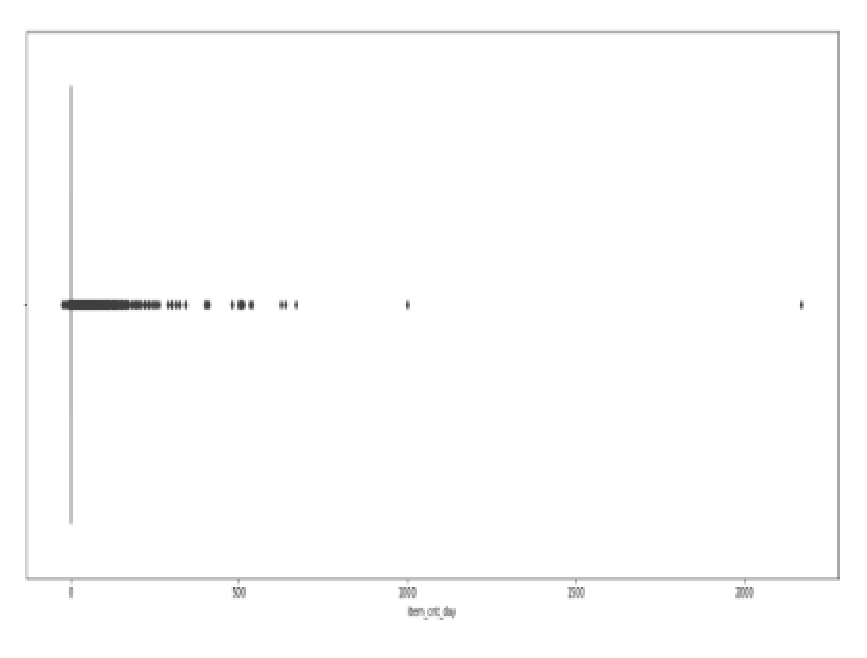
\includegraphics[width=0.6\textwidth]{figures//count.eps}\\
  \caption{C}\label{Distribution of sales}
\end{figure}
}{
\begin{figure}
  \centering
  \selectcolormodel{rgb}
  \missingfigure{Testing.}
  %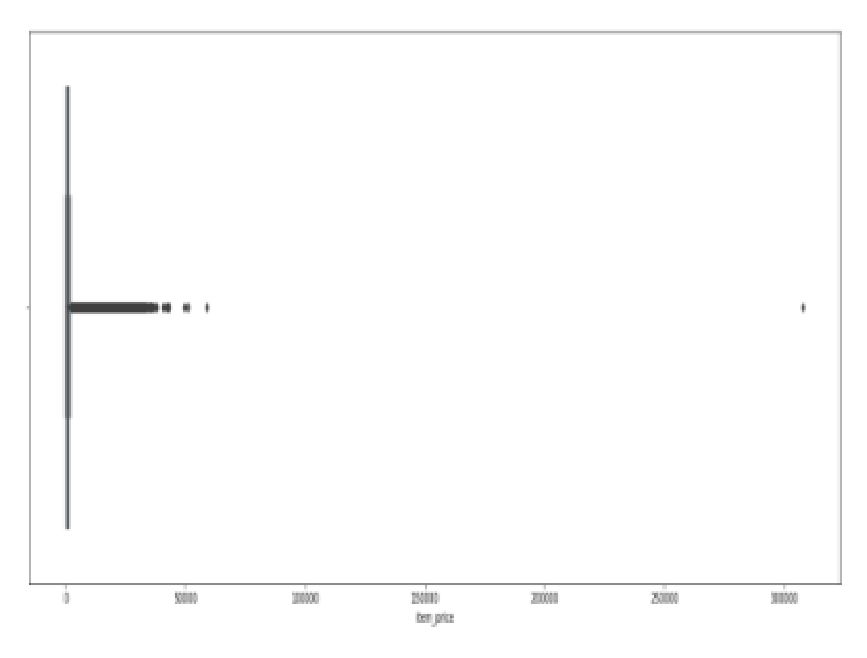
\includegraphics[width=0.6\textwidth]{figures//price.eps}\\
  \caption{P}\label{Price distribution}
\end{figure}
}

%%==========================================================================================
\begin{note}
However,
there is such a phenomenon in real life.
Doctors desire to identify the characteristics between
a group of cancer patients and normal people.
NBA coaches are passionate about exploring the obvious strengths and
weaknesses of the team compared with other teams.

Based on such a phenomenon in the real life,
we proposed the concept of group outlying aspects mining.
\end{note}
%%==========================================================================================

\end{slide}
%%
%%==========================================================================================


%%==========================================================================================
%%

\section{Data Visualization}


%%==========================================================================================
%%
\begin{slide}[toc=,bm=]{data visualization}
\begin{itemize}
 
\item
\textcolor{orange}{To predict next month's sales, find out how other factors affect sales}

\begin{itemize}
\item
Draw a bar chart according to the category, and the highest selling product is No. 40.

\item
Take 12 months as the observed value and draw the trend of monthly mean and sample standard deviation.

\item
Plot monthly mean sales and monthly mean standard deviation.
\end{itemize}
\end{itemize}

\begin{figure}[htbp]
    \centering
    \subfigure[Original Feature Spaces]{
      \selectcolormodel{rgb}
      \missingfigure[figwidth=5.5cm]{Test.}
        %\includegraphics[width=0.3\textwidth]{figures//example-basketball-original.eps}
        \label{fig:basketball-original}
    }
    \subfigure[Group Outlying Spaces]{
       \selectcolormodel{rgb}
       \missingfigure[figwidth=5.5cm]{Test.}
        %\includegraphics[width=0.3\textwidth]{figures//example-basketball-projection.eps}
        \label{fig:basketball-projection}
    }
    \subfigure[Another Subspaces]{
      \selectcolormodel{rgb}
      \missingfigure[figwidth=5.5cm]{Test.}
        %\includegraphics[width=0.28\textwidth]{figures//basketball-another-subspaces.eps}
        \label{fig:basketball-projection1}
    }
%    \caption{Histogram representation of a group on three single features}
    \label{fig:Basketball-Example}
\end{figure}

%%==========================================================================================
\begin{note}
We use $\rho_s(\cdot)$ to describe an outlying scoring function.
$\rho_s(\cdot)$ quantifies the outlying degree of the query group in a subspaces $s$.
In addition,
we use the scoring function to make a descending order and at last
filter out the top k group outlying subspaces.
It is obvious that the outlying subspaces make the
query group different from other groups.
\end{note}
%%==========================================================================================

\end{slide}
%%
%%==========================================================================================


%%==========================================================================================
%%
\begin{slide}[toc=,bm=]{Information acquired}
\begin{itemize}
\item
Item 40 sells the most.


\item
The sales volume in December and 24 months with obvious peak is judged to be the peak in the annual cycle.

\item
The monthly mean shows a decreasing trend, indicating that commodities have been declining on an annual basis.
\item
The sample variance increased month by month, indicating that the sales volume declined from the beginning of the second year to the beginning of the second year before stabilizing the downward trend.
\end{itemize}

%%==========================================================================================
\begin{note}
In order to identify the top-k outlying subspaces,
we categorize the features into $2$ non-overlapping groups,
trivial outlying features and non-trivial outlying subspaces.

First, let me introduce the trivial outlying features.

Trivial outlying features are one-dimension subspaces.
In the subspace,
the query group's outlying degree is larger than the threshold $\alpha$.

We can see from table $1$,
when the specified threshold $\alpha = 4$,
the trivial outlying feature is \{$F_1$\}.
\end{note}
%%==========================================================================================

\end{slide}
%%
%%==========================================================================================


%%==========================================================================================
%%


%%==========================================================================================
% TODO: Contact Page
\begin{wideslide}[toc=,bm=]{Contact Information}
\centering
\vspace{\stretch{1}}
\twocolumn[
lcolwidth=0.35\linewidth,
rcolwidth=0.65\linewidth
]
{
% \centerline{
\includegraphics[scale=.2]{tulip-logo.eps}}
}
{
\vspace{\stretch{1}}
Thank you for listening!\\
Siyu Chen\\
Xi'an Shiyou University\\
\begin{description}
 \item[\textcolor{orange}{\faEnvelope}] \href{mailto:785987165@qq.com}
 {\textsc{\footnotesize{785987165@qq.com}}}

 
\end{description}
}
\vspace{\stretch{1}}
\end{wideslide}

\end{document}

\endinput
